\section{Own Experiments}
\label{own-experiments}


\end{multicols}

\begin{figure}
    \centering
    \begin{subfigure}[b]{0.4\textwidth}
    \caption{}
        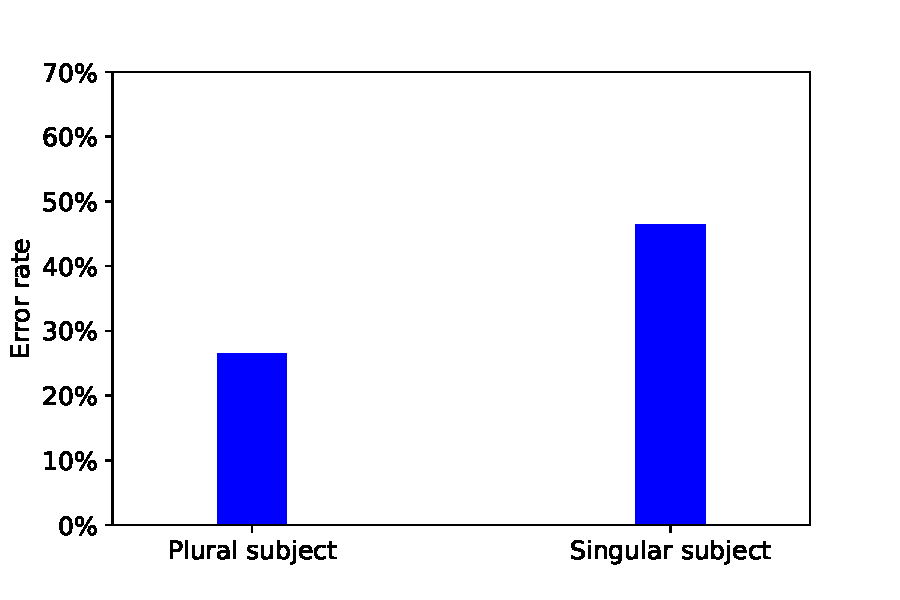
\includegraphics[width=\textwidth]{2b_least.pdf}
        \label{fig:2b_least}
    \end{subfigure}
    ~ %add desired spacing between images, e. g. ~, \quad, \qquad, \hfill etc. 
      %(or a blank line to force the subfigure onto a new line)
    \begin{subfigure}[b]{0.4\textwidth}

    \end{subfigure}
    \caption{\ref{fig:2b_least} shows the error rates of the language model for the least frequent nouns in the corpus as the subject and when no intervening nouns are present}
\end{figure}

\begin{multicols}{2}


To predict the correct number of a given verb,
the language model should be able to
1. identify the noun that is the head of the subject for the verb
2. establish the number of the noun (non-trivial since no knowledge of -s postfix for plurals)
3. establish the number of the given verb forms (also non-trivial).

In the first sub section we investigate if our model is able to
do this for simple cases with only a single noun in the prefix.
%
In the second sub section we investigate if our model can handle
more complex cases with two nouns in the prefix,
and what information it then uses to identify the head of the subject.

TODO: describe model (or in previous section)

\subsection{Noun-Verb Agreement in Simple Cases}


In this section we investigate the ability of the model to
establish number agreement for nouns and verbs in the simplest case,
following the pattern: ``The <noun> <verb>''. Notice that
the determiner ``The'' clearly indicates the position of the noun.

1. TEST DATA: 
Generate 100 x 50 simple prefixes in singular and plural form, like ``the company ... [produce/produces]'' 
and ``the companies ... [produce/produces]''.
The sentences do not need to be meaningful.
(randomly pick the nouns and verbs without taking into account their frequency in training data)

2. EXPERIMENT: 
Evaluate how the language model performs on these sentences 
and conclude whether or not the model is sensitive to noun-verb agreement in simple cases. 
(i.e. if it tends to predict plural verbs for plural nouns and singular verbs for singular nouns)
output 1: cross table with correct vs predicted
output 2: overall error rate number, error rate number for plurals, error rate number for singulars 


2. FURTHER ANALYSIS:
- Build a matrix: Nouns x Verbs, 
the entries tell whether the model predicted singular(1)
or plural(0).

- Sort the columns based on their sum
- Sort the rows for singular nouns based on their sum (upper half)
- Sort the rows for plural nouns based on their sum (lower half)
- print as an image (black = plural prediction, white is singular prediction)

- Discuss the picture:
  - Do we see verbs that clearly prefer singular resp. plural?
      (what is their plurality ratio?)
  - Do we see nouns that clearly prefer singular resp. plural
      (i.e. the model established their plurality), 
    or nouns that more or less follow the preference of the verbs?
     what is their frequency (count) in training corpus?)
  - Do we see nouns for which the model thinks
    that they are plural while they are in fact singular?
    
- Idea 1:
  - also include picture which shown models uncertainty in grey teints
    (uncertainty = evaluate(produces)/(evaluate(produce) + evaluate(produces))
    this is instead of max(evaluate(produces), evaluate(produce))

- Idea 2:
  - print noun counts as an y-axis
  - print verb plurality rates as an x-axis
  [other way to look at it: calculate unigram probs and normalize]
  (both are one dimensional matrices)
  (helps visualize these characteristics)
  (expectation: plurality rates decrease from left to right)
  (expectation: nouns in the middle appear less frequent in training corpus)
  (expectation: more plurality in upper half, resp. singularity in lower half. That is higher error rate)

- Idea 3:
  - repeat experiment for least frequent nouns
  (Is ordering of columns more or less the same?)
  (does the pattern looks different now?)
  
- Idea 4:
(might be very interesting)
- fill the noun verb matrix with co-occurence counts for
sentences of the training corpus (noun before verb).
Entries, for example for 'company and 'produce':
Count('company and produce co-occur')
normalize (i.e rescale such that all entries between zero and one)
Again, plot as an image.
Idee: maybe co-occurrences of singulars are high for regions
were model incorrectly predicts singular instead of plural.
  




%hypothesis: the model falls back to pure frequencies of the two verb forms
%in case it failed to learn the counts because of sparsity in the data.

%Further inspect the error cases, why did it fail for these very simple sentences:
%a) maybe the model failed to learn the number of the noun (i.e. low occurrence in training data for the given noun form)?
%b) maybe the model failed to learn the number of the verb forms (i.e. low occurrence in training data for both verb forms)?
%c) maybe the occurence in the training data of the incorrect but predicted verb form is much higher than the occurrence 
%in training data of the correct form?
%output a: histogram with x-axis z-score noun, y axis count (or percentage) of verbs that fall in this range
%output b: histogram with x-axis z-score verb (max of both), y axis count (or percentage) of verbs that fall in this range
%output c: histogram with x-axis percentage of predicted form, y axis count (or percentage) of verbs that fall in this range
%output(?): a scatter plot, x-axis z-score noun vs y-axis z-score verb, color gradient is percentage of predicted verb form

 
\subsection{Noun-Verb Agreement in Complex Cases}

In Section \ref{replication} we analysed the performance of the model
on complex sentences, containing one or more 
nouns.
The results show that the model is very
sensitive to the most recent noun,
performing worse-than-chance with only one single attractor.
%(Figure \ref{fig:2c}). 

In this section we investigate whether
syntactic and semantic information
can still help the model 
to establish number agreement
in case of multiple nouns.
We focus on sentences with exactly two nouns
of opposite number.


\subsubsection{Syntactic Information}

%%%%% OBJECTIVE
Function words such as `that' or `of' carry 
important information about the syntactic structure of a sentence.
In this Section we investigate if the model
uses this information to establish number agreement
for complex sentences.

%%%% TEST DATA
We generated sets of sentence prefixes using 
different syntactic templates.
An example is ``The \_ of the \_''
We instantiate these templates by randomly
picking two nouns and a verb 
from a set of frequently used nouns and verbs. 
Each combination of nouns and verbs instantiates
two prefixes that differ by their plurality.
For example ``The company of the governments''
and ``The companies of the government'',
with the option to choose between the verb forms
`know' and `knows'.
Since the nouns and verbs are randomly picked,
the generated prefixes 
are typically not semantically
meaningful.

We generated 2 x 1000 sentences per template,
for a total of 11 templates.
The sentences for each template are constructed using the same
noun and verb combinations.
We defined 7 templates for which the first noun is 
the head of the subject (table \ref{tab:attractor_templates}),
while 4 templates have the second noun as the head of the subject
(table \ref{tab:lastnoun_templates}).
The templates were defined after a manual inspection
of sentences from the corpus.

%%%% EXPERIMENT:
We evaluate how the model responds to the generated test inputs.
That is, for each test prefix we let the model decide between 
the singular and plural form of the given verb. 
We measure the error rate for each template.
However, instead of showing the error rates we
show how much the language model tends to agree with the most recent noun.
This corresponds to the error rate for the templates in table \ref{tab:attractor_templates},
while it corresponds to accuracy for the templates in table \ref{tab:lastnoun_templates}.
Showing the `last noun agreement rate' makes it easier
to compare the behavior of the model for different templates.

%%%% ANALYSIS:
The results are shown in Figure \ref{fig:last_noun_rates},
using green and red colors to indicate if 
the last noun is actually the head of the subject (green)
or not (red). 
%
We see that all bars are above the 0.5 rate,
which shows that the model is most
likely to agree with the last noun,
even in cases where this is syntactically incorrect. 
%
We also see that the red bars are slightly
lower than the green bars,
0.67 compared to 0.79 on average.
This shows that the model is even more likely
to prefer the last noun if this is
also syntactically correct.
This suggests that the model has 
at least some sensitivity
to syntactic information carried by function words.
%

%
We further discuss two special cases,
namely the first red bar (T1) and 
the last green bar (T11).
T1, ``the \_ and the \_ '', is a special case because it 
actually contains two singular nouns
instead of one singular and one plural noun. 
The predicted verb should be plural because of the
conjunction word `and'.
The existence of two singular nouns 
makes it hard for the model
to pick the plural verb,
which could explain the high error rate
for T1 in Figure \ref{fig:last_noun_rates}.
%
T11 uses different templates for the singular 
(the \_ 's \_ ) and the plural (the \_' \_) possessive form.
The last green bar in Figure \ref{fig:last_noun_rates} shows the average result.
We suspect that the relatively low accuracy
in this case might be explained by the infrequent
occurrence of the plural possessive form in written text.
Indeed, a closer inspection of the numbers showed that
the singular template had an accuracy
of 0.77 (compared to 0.71 for all singular prefixes), 
while the accuracy of the plural template
was lower, namely 0.66 (compared to 0.63 overall for plural prefixes).
%

%%%% DISCUSSION / CONCLUSION:
We conclude that, although the model 
performs poorly on syntactically complex sentences it
still shows some sensitivity for syntactic 
information exposed by function words. 


\begin{Figure}
    \centering

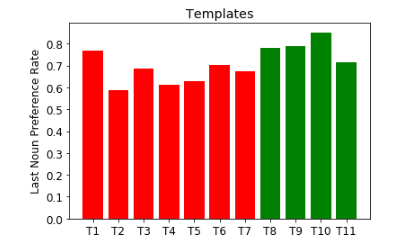
\includegraphics[scale=0.5]{screenshot-syntactic-templates} 
\captionof{figure}{Preference rates for agreement to the last noun.
The colors indicate whether this is syntactically correct (green)
or incorrect (red).
}
%TODO: save picture instead of making screenshot 
%TODO title Templates below
\label{fig:last_noun_rates}
\end{Figure}


\end{multicols}{2}



 
\begin{table}[t] 
\parbox{.45\linewidth}{
\centering
\begin{tabular}{ l l r }
  T1    & the \_ and the \_     &  0.77 \\
  T2    & the \_ in the \_      &  0.59 \\
  T3    & the \_ by the \_      &  0.69 \\
  T4    & the \_ of the \_      &  0.61 \\
  T5    & the \_ near the \_    &  0.63\\
  T6    & the \_ at the \_      &  0.70\\
  T7    & the \_ without the \_ & 0.67  \\
\end{tabular}
\caption{Templates for which the number of the verb 
is opposite to the number of the last noun} 
\label{tab:attractor_templates}
}
\hfill
\parbox{.45\linewidth}{
\centering
\begin{tabular}{ l l r }
  T8    & the \_ the \_         &  0.78\\
  T9    & the \_ that the \_    &  0.79\\
  T10   & the \_ whether the \_ &  0.85\\
  T11   & the \_ 's \_ (for plural: the \_' \_)          &  0.72 \\
\\
\\
\\
\end{tabular}
\caption{Templates for which the number of the verb 
corresonds to the number of the last noun} 
\label{tab:lastnoun_templates}
}
\end{table}

\begin{multicols}{2}


\subsubsection{Semantic Information}

We now look at semantic clues, i.e. companies
are more likely to produce than employees.
We investigate if the model is able to establish
number agreement between the verb and the semantic related noun,
ignoring the non-semantic related attractor noun.
  
1. TEST DATA:
We construct a testset (100+ sentences) consisting of pairs with singular and plural prefixes, in the following format  
``The NN of the NNS ...[VBZ/VBP]'' and
``The NNS of the NN ...[VBZ/VBP]'' 
whereby the head of the subject (the first noun)
is semantically related to the verb, while the attractor (the second noun)
is randomly picked. An example is:
``The prices of the employee ...[stabilizes/stabilize]'' and 
``The price of the employees ...[stabilizes/stabilize]''.

In addition we construct a comparison set consisting of the same prefixes
(same verb and attractor noun),
but with the difference that the first noun is also randomly picked and
therefore most likely not semantically related. Example:
``The newspapers of the employee ...[stabilizes/stabilize]'' and 
``The newspaper of the employees ...[stabilizes/stabilize]''.


EXPERIMENT:
Evaluate our model on the constructed testset and on the comparison set.
If the model scores significantly better on the testset
then it shows sensitivity to semantic clues.

%(remark: we can repeat the experiment with the nouns interchanged and check that we %score worse now,
%e.g. "The employee that the prices ... [stabilize/stabilizes]" 
%In that case syntax and semantics are inconsistent)

HOW TO FIND CO-OCCURRENCE RATIOS
\begin{itemize}
\item find all nouns (NN) and verbs (VBZ) in a tagged corpus 
(sec02-21.gold.tagged).
(pick a random selection if all is too much
but make sure you are not only looking at
frequent verbs since they tend to be general like 'is/are'
instead of specific like 'stabilize')
\item  build a matrix with nouns as rows and columns as verbs
\item  fill entries with Count('noun and verb co-occur in a sentence')
i.e. loop over all sentences and add one if noun and verb exists in sentence
\item  divide all entries by their column total
\item select for each column the entry with the highest score(s)
(you may ignore very general verbs like is/are)
\end{itemize}

Remark: the semantically related noun/verb combinations can also be manually
chosen, but learned from data is preferable. 
'frequently occur together' means: count(VBZ + NN)/count(VBZ) is 
relatively high.

Remark: can be learned from tagged data set, no need to look at training data

Remark: Interesting reading about similarity metrics https://web.stanford.edu/~jurafsky/slp3/15.pdf